\documentclass[11pt]{article}
\usepackage[a4paper,margin=1in]{geometry}
\usepackage{amsmath,amssymb}
\usepackage{booktabs,tabularx}
\usepackage{enumitem}
\usepackage[table]{xcolor}
\usepackage{tikz}
\usetikzlibrary{arrows.meta,positioning,fit,backgrounds}
\usepackage{microtype}
\usepackage[font=small,labelfont=bf]{caption}
\usepackage[colorlinks=true,linkcolor=black,urlcolor=black,citecolor=black]{hyperref}
\usepackage{xurl}

\definecolor{pulse}{HTML}{2E7D55}
\definecolor{ink}{HTML}{1B211D}
\definecolor{warnred}{HTML}{C2412D}
\definecolor{soft}{HTML}{EEF6F1}

\newcommand{\code}[1]{\texttt{\small #1}}
\setlist{itemsep=2pt,topsep=4pt}
\emergencystretch=3em
\sloppy

\title{\textbf{PULSE: A Provenance-First Identity Layer for\\Tokenized Real-World Assets}}
\author{Project PULSE\\[2pt]
\small Build with CMC: API Hackathon --- Real World Assets track\\
\small September 30, 2026 \textperiodcentered{} Data: CoinMarketCap Pro API, live\\
\small Source: \url{github.com/notwen123/PULSE}}
\date{}

\begin{document}
\maketitle

\begin{abstract}
\noindent A tokenized real-world asset reaches a user as a ticker, and a ticker is not an instrument. In live CoinMarketCap data, the symbol \code{TSLA} fans out to nine distinct on-chain tokens minted by eight issuers across thirteen chains --- one of which CoinMarketCap returns with no price at all. Existing interfaces present such tokens as prices; none presents them as identities, and none says where a displayed number came from. We present \textsc{PULSE}, a verification layer that resolves any ticker or name to a stable CoinMarketCap \code{rwa\_id}, composes an \emph{RWA Passport} relating the underlying asset to every issuer, token representation, and chain, and attaches to every important value a \emph{data receipt}: the exact endpoint and JSON field, the source timestamp, the retrieval time, the credit cost, and a SHA-256 fingerprint of the canonicalized response. The system's central invariant is that \emph{no value is displayed without provenance and no absent value is displayed at all}: a field CMC omits renders as unavailable, never as a fabricated number, and fixture data can never carry a \emph{verified} status. A Passport costs at most four CMC calls; identity resolution costs zero credits. The same receipts are exposed as JSON through an Evidence API so that automated agents can verify an answer rather than merely restate it. The reference implementation is 4,903 lines of TypeScript on Next.js~16 with 31 passing tests, and every endpoint it depends on was verified against the live Pro API: ten of ten returned HTTP~200, totalling nine credits per full capture. We report what we measured, including six places where live responses diverged from published examples.
\end{abstract}

\noindent\textbf{Keywords:} real-world assets; tokenization; data provenance; identity resolution; CoinMarketCap API; verifiable interfaces; agent tooling.

\section{Introduction}

Tokenization moves equities, commodities, treasuries and funds onto public chains, and it does so many times over. The same company can be represented by several issuers, each minting its own token, each deployed to its own set of chains, each with its own liquidity and price. CoinMarketCap now tracks 7,942 tokenized real-world assets from 25 issuers. The ticker a user searches for collapses all of this into a single string.

Two failures follow. The first is \emph{identity}: a user who sees \code{TSLAX}, \code{TSLA.D}, \code{rTSLA} and three tokens all named \code{TSLA} cannot tell, from the interface, that they share an underlying asset, who issued each one, or where each one lives. The second is \emph{provenance}: when an interface shows a price, it rarely says which data source produced it, when that source last updated, or whether the number exists at all. In the data we measured, one Tesla representation has \code{price: null}. An interface that renders it as \$0.00, or silently drops it, tells the user something false.

\textsc{PULSE}'s position is that both failures are interface failures, not data failures. CoinMarketCap's RWA API already introduces a stable identifier for the asset itself (\code{rwa\_id}), separate from the \code{crypto\_id} of each token, and its quotes endpoint already returns the tokens behind an asset with their issuers. What is missing is a layer that makes the relationships visible and keeps every number attached to its source. We build that layer and hold it to one discipline: verify against the live API, display only what was returned, and say so when something was not.

The claim is deliberately narrow. \textsc{PULSE} explains and verifies data; it does not recommend trades, score issuer risk, or claim venue-level price coverage. Market-pair data (\code{/v5/real-world-assets/market-pairs/list}) is available only on Growth plans and above and is not used. A response fingerprint proves which payload a value came from; it does not prove that the market value is correct, and the interface says exactly that.

\subsection{Contributions}
\begin{itemize}
\item An identity-first resolution pipeline that maps any ticker or name to a stable \code{rwa\_id} through CMC's zero-credit RWA ID Map, with a deterministic ranking over exact, prefix and name matches (Sections~3--4).
\item The RWA Passport: a composition of metadata, tokenized aggregate, token representations, issuers and chains in at most four CMC calls, with no per-token or per-issuer fan-out (Section~4.2).
\item A per-value receipt construction --- endpoint, query, JSON field path, identifier, source and retrieval timestamps, credit count, and a SHA-256 fingerprint of a canonical serialization --- with a status function under which fixture data can never present as verified (Sections~4.3--4.4).
\item An Evidence API that returns the same receipts as structured JSON for scripts and AI agents (Section~6).
\item An evaluation against the live Pro API and six documented divergences between published examples and live responses, each of which changed the implementation (Sections~7--8).
\end{itemize}

\section{Problem Statement and Design Goals}

We consider four principals: the \emph{user}, who searches by ticker or name and acts on what is displayed; the \emph{browser}, untrusted for secrets; the \emph{PULSE server}, trusted for integrity of its own pipeline and sole holder of the API key; and \emph{CoinMarketCap}, trusted as the source of record for the data it returns but not assumed to return every field.

\textbf{Goals.} (G1) \emph{Identity before price:} every asset view is keyed by \code{rwa\_id}, never by ticker. (G2) \emph{Provenance totality:} every displayed key value carries a receipt naming its endpoint, field and timestamps. (G3) \emph{No fabrication:} a field absent from the response renders as unavailable; no value is synthesized, interpolated or defaulted to zero. (G4) \emph{Honest modes:} fixture data, used only when no key is configured, is labelled on every surface and can never carry a \emph{verified} status. (G5) \emph{Bounded cost:} a Passport costs a constant number of calls independent of how many tokens an asset has. (G6) \emph{Graceful degradation:} each data source fails independently; one unavailable endpoint never blanks a page. (G7) \emph{Secret isolation:} the API key never reaches the browser, logs, receipts or evidence files.

\textbf{Non-goals.} Investment advice, trading signals or issuer risk scores; venue-level price discovery (Market Pairs, Growth+); historical series, which the documented RWA endpoints do not provide; and proving that a market value is correct, as opposed to proving which response it came from.

\begin{figure}[t]
\centering
\resizebox{\linewidth}{!}{%
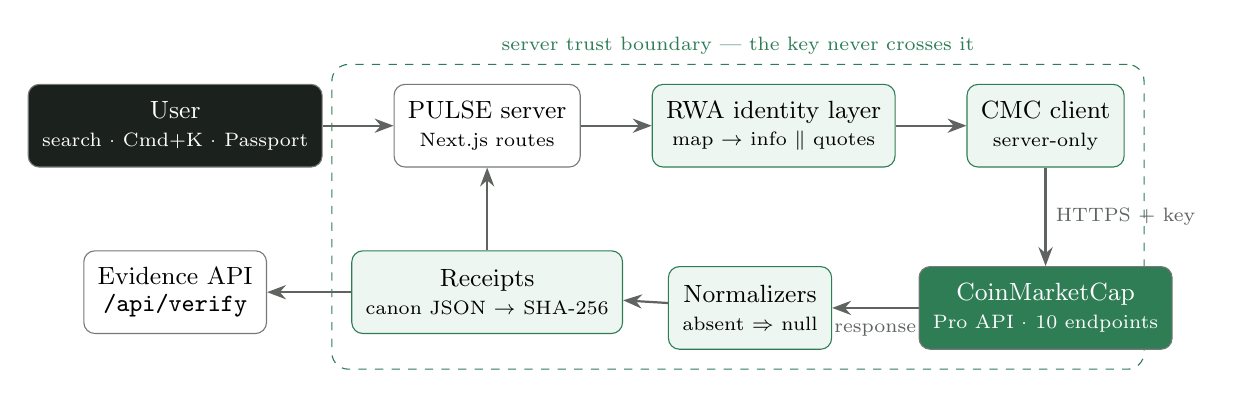
\begin{tikzpicture}[
  font=\small,
  box/.style={draw=ink!60,rounded corners=4pt,fill=white,align=center,minimum height=1.05cm,inner sep=5pt},
  core/.style={box,fill=soft,draw=pulse},
  arr/.style={-{Stealth[length=2.4mm]},thick,ink!70},
  >=Stealth]
\node[box,fill=ink,text=white] (user) {User\\[-1pt]\scriptsize search \textperiodcentered{} Cmd+K \textperiodcentered{} Passport};
\node[box,right=0.9cm of user] (next) {PULSE server\\[-1pt]\scriptsize Next.js routes};
\node[core,right=0.9cm of next] (rwa) {RWA identity layer\\[-1pt]\scriptsize map \(\to\) info \(\parallel\) quotes};
\node[core,right=0.9cm of rwa] (cli) {CMC client\\[-1pt]\scriptsize server-only};
\node[box,fill=pulse,text=white,below=1.25cm of cli] (cmc) {CoinMarketCap\\[-1pt]\scriptsize Pro API \textperiodcentered{} 10 endpoints};
\node[core,below=1.25cm of rwa,xshift=-0.3cm] (norm) {Normalizers\\[-1pt]\scriptsize absent \(\Rightarrow\) null};
\node[core,below=1.05cm of next] (rcpt) {Receipts\\[-1pt]\scriptsize canon JSON \(\to\) SHA-256};
\node[box,below=1.05cm of user] (ev) {Evidence API\\[-1pt]\scriptsize \code{/api/verify}};
\draw[arr] (user) -- (next);
\draw[arr] (next) -- (rwa);
\draw[arr] (rwa) -- (cli);
\draw[arr] (cli) -- node[right,font=\scriptsize]{HTTPS + key} (cmc);
\draw[arr] (cmc) -- node[below=2pt,font=\scriptsize]{response} (norm);
\draw[arr] (norm) -- (rcpt);
\draw[arr] (rcpt) -- (ev);
\draw[arr] (rcpt) -- (next);
\begin{scope}[on background layer]
\node[draw=pulse,dashed,rounded corners=6pt,fit=(rwa)(cli)(norm)(rcpt),inner sep=7pt,label={[font=\scriptsize,text=pulse]above:server trust boundary --- the key never crosses it}] {};
\end{scope}
\end{tikzpicture}}
\caption{\textsc{PULSE} architecture. The identity layer composes CMC responses; normalizers convert them into stable types without inventing absent fields; every displayed value carries a receipt derived from the response it came from. The browser and agents see only normalized values and receipts.}
\label{fig:arch}
\end{figure}

\section{System Architecture}

\textsc{PULSE} is a Next.js~16 application (React~19, TypeScript) in which every CoinMarketCap call is made by a single server-only client module; importing it from client code fails the build. The client applies a 7-second timeout, at most two attempts, exponential backoff (300\,ms base for network errors, 500\,ms for transient HTTP failures), honours \code{Retry-After} up to five seconds, and maps both HTTP status and CMC's \code{status.error\_code} to a closed set of error kinds (Table~\ref{tab:errors}). It logs endpoint and error kind only, never the key or the upstream body.

\subsection{Why identity is resolved before price}
A ticker search answers \emph{which string matches}; an \code{rwa\_id} answers \emph{which asset is meant}. CMC's own guidance recommends \code{rwa\_id} over symbols, and the distinction is concrete in the data: the SpaceX example in CMC's documentation notes that \code{SPCX} refers to both a Nasdaq listing and a tokenized asset. \textsc{PULSE} resolves first, through the RWA ID Map (0 credits), and keys every subsequent call and every URL (\code{/passport/14}) on the resolved identifier. A user can share a Passport link without the ambiguity a ticker carries.

\subsection{Why receipts are per value rather than per page}
A page-level ``data from CoinMarketCap'' credit is unfalsifiable. A per-value receipt is checkable: it names the field path inside the response, the parameters sent, and a fingerprint of the bytes received, and it includes a reproducible \code{curl} command with the key elided. A typical field path is
\begin{center}\code{data.rwa\_assets[0].quotes[0].average\_tokenized\_price}\end{center}
Because receipts are derived from response metadata rather than authored, a value cannot carry a receipt for a response it did not come from.

\section{The Resolution and Evidence Calculus}

\subsection{Resolution}
Let \(M\) be the set of map records returned for a query \(q\), each with symbol \(s\), name \(n\), slug \(g\) and rank \(\rho\). For lowercased \(q\) we define a match score
\begin{equation}
\sigma(a,q)=\begin{cases}
0 & s = q\\
1 & q \text{ is a prefix of } s\\
2 & q \text{ is a prefix of } n\\
3 & q \subseteq n \;\lor\; \mathrm{kebab}(q) \subseteq g\\
\bot & \text{otherwise,}
\end{cases}
\label{eq:rank}
\end{equation}
and return candidates with \(\sigma\neq\bot\) ordered lexicographically by \((\sigma,\rho)\), deduplicated by \code{rwa\_id}. Ticker-shaped queries (\code{[0-9A-Za-z\$@-]\{1,15\}}) first hit the map with \code{symbol=}\(q\) (exact, 0 credits); name queries such as ``Apple'' or ``Silver'' are matched against a cached index of the top 1,000 assets by rank (four pages of 250, refreshed hourly, 0 credits).

\subsection{Passport composition}
For a resolved \(r\), the Passport is
\begin{equation}
P(r) \;=\; \underbrace{\mathrm{info}(r) \parallel \mathrm{quotes}(r)}_{\text{parallel}} \;\to\; \mathrm{cryptoInfo}\big(\{c_i\}\big) \;\parallel\; \mathrm{issuers}(\cdot),
\label{eq:passport}
\end{equation}
where \(\{c_i\}\) are the \code{crypto\_id}s of the tokens returned by quotes, fetched in a single batched call, and \(\mathrm{issuers}(\cdot)\) is the issuer directory (one call, cached 15 minutes). The token-to-issuer relation is read directly from \code{tokens[].issuer\_id}; no per-issuer request is made. Hence the call count is bounded by
\begin{equation}
|\mathrm{calls}(P(r))| \le 4 \quad\text{independent of the number of tokens,}
\end{equation}
which satisfies G5. Secondary failures (chain metadata, issuer directory) degrade to a warning on the page; only a failure of \(\mathrm{info}(r)\) prevents a Passport from rendering.

\subsection{Currency selection}
With \code{convert=}\(C\), live responses nest the converted aggregate in an array \(Q=\code{quotes[]}\) while the flat fields remain in USD. The selected block is
\begin{equation}
\beta(x,C)=\begin{cases}
Q_j & \exists j: Q_j.\mathrm{symbol}=C\\
x.\mathrm{quote}[C] & \text{if present}\\
x \ (\text{labelled USD}) & \text{otherwise,}
\end{cases}
\end{equation}
and the returned currency label is the one actually used, never the one requested. Token prices are returned in USD regardless of \(C\); the Passport labels them as such rather than presenting them in the requested currency.

\subsection{Receipts and fingerprints}
A receipt for a value \(v\) extracted from response \(\mathcal{R}\) is the tuple
\begin{equation}
\mathsf{receipt}(v)=\big(e,\ \pi,\ f,\ \iota,\ v,\ t_{\mathrm{ret}},\ t_{\mathrm{src}},\ \kappa,\ h,\ \mathsf{status}\big),
\end{equation}
with endpoint \(e\), query parameters \(\pi\) (excluding credentials), field path \(f\), identifier \(\iota\) (\code{rwa\_id} or \code{crypto\_id}), retrieval time \(t_{\mathrm{ret}}\), source time \(t_{\mathrm{src}}\) (the record's own \code{last\_updated} when present, else \code{status.timestamp}), credit count \(\kappa\) from \code{status.credit\_count}, and fingerprint
\begin{equation}
h=\mathrm{SHA\mbox{-}256}\big(\mathrm{canon}(\mathcal{R})\big),
\end{equation}
where \(\mathrm{canon}\) serializes objects with keys sorted lexicographically at every depth, preserves array order, and omits \code{undefined} members. Canonicalization makes \(h\) independent of key order, so two receipts share a fingerprint if and only if they came from the same payload. The status function is
\begin{equation}
\mathsf{status}(v)=\begin{cases}
\textsf{unavailable} & v=\mathtt{null}\\
\textsf{demo} & \text{mode}=\text{fixture}\\
\textsf{verified} & \text{otherwise.}
\end{cases}
\label{eq:status}
\end{equation}
The ordering in Eq.~\ref{eq:status} is load-bearing: an absent value is never \emph{verified}, and fixture data is never \emph{verified} regardless of its content. Table~\ref{tab:receipt} lists what each receipt field forecloses.

\begin{table}[t]
\centering\small
\begin{tabularx}{\linewidth}{@{}lX@{}}
\toprule
Receipt field & Forecloses\\
\midrule
Endpoint + query & An unfalsifiable ``data from CMC'' credit\\
JSON field path & A value attributed to the wrong field of a correct response\\
Identifier (\code{rwa\_id}/\code{crypto\_id}) & A price shown against the wrong asset or token\\
Source vs.\ retrieval timestamp & Stale data presented as current\\
Credit count & Hidden cost of a call\\
SHA-256 of canonical response & Two values claimed to share a source when they do not\\
Status (Eq.~\ref{eq:status}) & Absent or fixture values presented as verified\\
Reproducible \code{curl} (key elided) & A receipt that cannot be independently re-run\\
\bottomrule
\end{tabularx}
\caption{Receipt fields and the failure each one forecloses.}
\label{tab:receipt}
\end{table}

\section{Data Sources}

Table~\ref{tab:endpoints} lists every endpoint the implementation calls, its role, and the cache window applied, chosen to match or exceed CMC's documented update frequency. Fear \& Greed and the Altcoin Season Index fall back to CMC's documented keyless \code{/public-api} prefix when no key is configured; all RWA endpoints require a key.

\begin{table}[t]
\centering\small
\begin{tabularx}{\linewidth}{@{}lXr@{}}
\toprule
Endpoint & Role in \textsc{PULSE} & Cache\\
\midrule
\code{/v5/real-world-assets/map} & Ticker/name \(\to\) \code{rwa\_id} (0 credits) & 5\,min / 1\,h\\
\code{/v5/real-world-assets/info} & Identity, description, company facts & 15\,min\\
\code{/v5/real-world-assets/quotes/latest} & Aggregate, tokens + issuers, TradFi & 60\,s\\
\code{/v5/real-world-assets/assets/list} & Ranked list of tracked RWAs & 60\,s\\
\code{/v5/real-world-assets/issuers/list} & Issuer directory & 15\,min\\
\code{/v5/real-world-assets/issuers} & Issuer \(\to\) tokens \(\to\) Passports & 15\,min\\
\code{/v2/cryptocurrency/info} & Chain/platform per token (batched) & 24\,h\\
\code{/v1/global-metrics/quotes/latest} & Market cap, volume, dominance & 5\,min\\
\code{/v3/fear-and-greed/latest} & Market sentiment & 15\,min\\
\code{/v1/altcoin-season-index/latest} & Market regime & 15\,min\\
\bottomrule
\end{tabularx}
\caption{CoinMarketCap endpoints used. Market Pairs (Growth+) is deliberately not used.}
\label{tab:endpoints}
\end{table}

\begin{table}[t]
\centering\small
\begin{tabular}{@{}lll@{}}
\toprule
Condition & Kind & Behaviour\\
\midrule
HTTP 401, \code{error\_code} 1001/1002 & \code{invalid\_key} & Fail, no retry\\
HTTP 402/403, codes 1005--1007 & \code{forbidden} & Fail, no retry\\
HTTP 429, codes 1008--1011 & \code{rate\_limited} & Retry once, honour \code{Retry-After} \(\le\)5\,s\\
HTTP 400 & \code{bad\_request} & Fail; on Passport \(\Rightarrow\) not found\\
HTTP 5xx / network error & \code{unavailable} & Retry once with backoff\\
Timeout (7\,s) & \code{timeout} & Retry once with backoff\\
\code{data} absent & \code{malformed} & Fail\\
\bottomrule
\end{tabular}
\caption{Error taxonomy of the CMC client. Every kind maps to user-facing copy and an HTTP status on the Evidence API; no kind exposes upstream bodies.}
\label{tab:errors}
\end{table}

\section{Evidence API}

\code{GET /api/verify?q=}\(k\) answers one of five structured queries --- \code{rwa-identity}, \code{rwa-quote} (by \code{symbol} or \code{rwa\_id}, optional \code{convert}), \code{fear-and-greed}, \code{altcoin-season}, \code{btc-dominance} --- with a natural-language answer and the full receipt: value, source, endpoint, parameters, field, identifier, retrieval time, CMC timestamp, response hash, credit count, verification status and data mode. The landing page renders the identical object, produced by the same function, so the example a reader sees is the shape an agent receives. \textsc{PULSE} does not proxy or replace CMC's own MCP server; it adds a provenance layer that an agent can call as a plain HTTP tool, turning ``the model said so'' into ``the model said so, and here is the response it came from''.

\section{Implementation and Evaluation}

The implementation comprises 4,903 lines of TypeScript, of which 1,750 form the data, normalization and receipt layers; ten API routes; nine pages; and 31 unit tests across three suites covering normalization of documented and live shapes, \code{rwa\_id} ranking, receipt construction, hash determinism, number formatting and null handling. Lint (ESLint + \code{tsc --noEmit}) and the production build pass.

\subsection{Live endpoint verification}
A capture script calls each endpoint with the configured key and writes the response, HTTP status, capture time and SHA-256 to \code{evidence/live/}; the key is sent only as a header and a post-capture scan confirms it appears in no file. Table~\ref{tab:live} reports the capture of September 30, 2026. CMC-reported \code{status.elapsed} is server-side processing time, not end-to-end latency, and is reported as such.

\begin{table}[t]
\centering\small
\begin{tabular}{@{}lccc@{}}
\toprule
Endpoint & HTTP & Credits & \code{elapsed} (ms)\\
\midrule
\code{/v5/real-world-assets/map} & 200 & 0 & 1\\
\code{/v5/real-world-assets/info} & 200 & 1 & 3\\
\code{/v5/real-world-assets/quotes/latest} & 200 & 1 & 5\\
\code{/v5/real-world-assets/assets/list} & 200 & 1 & 10\\
\code{/v5/real-world-assets/issuers/list} & 200 & 1 & 3\\
\code{/v5/real-world-assets/issuers} & 200 & 1 & 4\\
\code{/v2/cryptocurrency/info} & 200 & 1 & 11\\
\code{/v1/global-metrics/quotes/latest} & 200 & 1 & 11\\
\code{/v3/fear-and-greed/latest} & 200 & 1 & 2\\
\code{/v1/altcoin-season-index/latest} & 200 & 1 & 4\\
\midrule
Total & 10/10 & 9 & ---\\
\bottomrule
\end{tabular}
\caption{Live capture against the CoinMarketCap Pro API, September 30, 2026 (19:14 UTC).}
\label{tab:live}
\end{table}

\subsection{Case study: one ticker, nine instruments}
Resolving \code{TSLA} returns \code{rwa\_id}~14 (Tesla, Inc., rank~12). Its Passport, built from one quotes call and one batched chain lookup, relates the asset to nine token representations, eight issuers and thirteen chains through twenty-two token--chain links. The distribution is uneven: \code{TSLAX} (Backed Assets) is deployed to seven chains, while one token carries no chain metadata at all. One representation, \code{TSLA.D} (Dinari Assets, Arbitrum), is returned with \code{price: null}; under Eq.~\ref{eq:status} its receipt reads \textsf{unavailable} and the interface renders ``not in CMC data'' rather than a number. This single asset exhibits both failures from Section~1, and the Passport resolves both from data CMC already returns.

\subsection{Cost and latency}
A cold Passport costs at most four credits (info, quotes, chain metadata, issuer directory) and typically fewer, since the directory is shared across Passports for 15 minutes; identity resolution costs zero. A cached Passport was served in 22\,ms (time to first byte, local production build). With CMC unreachable from the development network, Daily Pulse streamed its first byte in 0.11\,s and resolved every degraded section to an explicit unavailable state after 14.3\,s (two attempts at the 7\,s timeout), rather than blocking the page.

\section{Findings from Testing Against the Live API}

The implementation was first written against CMC's published examples and then corrected against live responses. Each finding below changed code.

\begin{enumerate}
\item \textbf{Converted quotes are an array.} With \code{convert=EUR}, the converted aggregate arrives as \code{quotes: [\{symbol:"EUR",\,\dots\}]}; the flat aggregate fields remain in USD. A reader assuming a \code{quote.EUR} object, as the reference wording suggests, silently shows USD values labelled EUR.
\item \textbf{Token prices ignore \code{convert}.} \code{tokens[].price} is USD in every response we observed. The Passport labels token prices with the currency actually returned.
\item \textbf{Issuers are on the tokens.} Live \code{tokens[]} carry \code{issuer\_id} and \code{issuer\_name}, which the documented example omits. Our first implementation built a token\(\to\)issuer index by calling the Issuer endpoint once per issuer; the live shape let us delete that fan-out entirely and bound the Passport at four calls.
\item \textbf{TradFi rows have no price.} \code{tradfi\_markets[]} items are \code{\{exchange:\{name,\,slug,\,exchange\_id\},\,ticker,\,market\_url\}}; the documented example is an empty array. \textsc{PULSE} shows venue and a link, never an inferred price.
\item \textbf{Envelope types vary.} \code{status.error\_code} is the string \code{"0"} on the RWA and Fear \& Greed endpoints and the number \code{0} on the Altcoin Season Index; the Altcoin timestamp is \code{snapshot\_time}. An unknown \code{rwa\_id} on \code{/info} returns HTTP~400, not 404, which \textsc{PULSE} treats as not found.
\item \textbf{Coverage differs from category listings.} \code{asset\_type=government\_security} currently returns \code{total\_size: 0}, and for SpaceX (\code{rwa\_id}~9) \code{about.description}, \code{about.logo}, \code{primary\_exchange} and \code{cik} were \code{null}. \textsc{PULSE} hides null facts rather than filling them, and its demo prompts were changed from ``US Treasury'' to assets that exist.
\end{enumerate}

\section{Trust Assumptions and Limitations}
Stated plainly, in decreasing order of weight.
\begin{enumerate}
\item \textbf{The fingerprint is not a proof of truth.} It proves which payload a value came from and that two values share a source; it does not prove the market value is correct, and receipts say so.
\item \textbf{Name search covers the top 1,000 assets by rank.} Exact tickers resolve across the full catalogue; free-text names outside the cached index will not be found until the map offers a name parameter or the index is extended.
\item \textbf{No history or change data.} The documented RWA endpoints expose no historical series or 24-hour change on the aggregate; \textsc{PULSE} computes none and shows none.
\item \textbf{Chain coverage depends on \code{/v2/cryptocurrency/info}.} Tokens without platform metadata render as ``chain not in CMC data''.
\item \textbf{Fixture data exists for development.} Without a key, RWA pages use labelled fixtures based partly on CMC's documentation examples and partly on placeholders; every receipt then reads \textsf{demo} and no surface presents them as live.
\item \textbf{Saved assets are browser-local.} Watchlists and progress live in \code{localStorage}; they do not sync across devices by design, since the demo requires no account.
\end{enumerate}

\section{Related Work}
\textbf{Market-data aggregators} present tokens as prices and rank them by capitalization; \textsc{PULSE} sits on top of one such source and adds identity and per-value provenance rather than competing on coverage. \textbf{Block explorers} expose contracts and transfers per chain but have no notion of the underlying asset shared across issuers and chains. \textbf{RWA analytics platforms} aggregate market size by category; \textsc{PULSE} answers a different, per-asset question: \emph{what exactly is this token, and where did this number come from?} \textbf{Oracle networks} deliver attested values on-chain for contracts; \textsc{PULSE} delivers attested values to people and agents off-chain, with the attestation reduced to what a reader can check: endpoint, field, time and fingerprint. \textbf{Provenance models} such as W3C PROV formalize derivation records; our receipt is a deliberately minimal instance specialized to a single HTTP response.

\section{Future Work}
Server-side name search over the full catalogue; per-asset change tracking from snapshots \textsc{PULSE} itself records, labelled as derived; venue-level comparison when Market Pairs is available on the deployment plan; signed receipts so a fingerprint can be attributed to a specific \textsc{PULSE} deployment; and an MCP tool definition wrapping \code{/api/verify} for direct use by agent frameworks.

\section{Conclusion}
A ticker is a string; an asset is an identity; a number is a claim. \textsc{PULSE} keeps the three apart: it resolves the string to a stable CoinMarketCap identity, shows every instrument behind it, and attaches to each number the response it came from. The design rests on one discipline applied throughout: verify against the live API, display only what was returned, and label what was not. Every figure in this paper was measured under that discipline.

\begin{thebibliography}{9}\small
\bibitem{cmc-rwa} CoinMarketCap. \emph{Pro API Reference: Real World Assets} (\code{/v5/real-world-assets}). coinmarketcap.com/api/documentation, 2026.
\bibitem{cmc-rwa-landing} CoinMarketCap. \emph{RWA API --- Tokenized Stocks, Gold, and Treasuries.} coinmarketcap.com/api/real-world-assets-api, 2026.
\bibitem{cmc-spcx} CoinMarketCap. \emph{How to Pull SpaceX Real-World Asset Data From CoinMarketCap Pro API.} 2026.
\bibitem{cmc-global} CoinMarketCap. \emph{Pro API Reference: Global Metrics, Fear and Greed, Altcoin Season Index.} 2026.
\bibitem{fips} NIST. \emph{FIPS 180-4: Secure Hash Standard.} 2015.
\bibitem{jcs} Rundgren, A., Jordan, B., Erdtman, S. \emph{RFC 8785: JSON Canonicalization Scheme.} IETF, 2020.
\bibitem{prov} W3C. \emph{PROV-DM: The PROV Data Model.} W3C Recommendation, 2013.
\bibitem{mcp} Anthropic. \emph{Model Context Protocol Specification.} modelcontextprotocol.io, 2025.
\bibitem{pulse} Project PULSE. Source, tests and live evidence captures. github.com/notwen123/PULSE, 2026.
\end{thebibliography}

\vspace{6pt}
\noindent\rule{\linewidth}{0.4pt}\\
{\footnotesize \textsc{PULSE} is hackathon software. Endpoint results in Table~\ref{tab:live} were captured from the CoinMarketCap Pro API on September 30, 2026 by \code{scripts/capture-evidence.mjs}; raw responses with their SHA-256 are in \code{evidence/live/}. The case-study figures were read from the live Passport for \code{rwa\_id}~14 on the same day. Code metrics were measured at the commit tagged for submission. Nothing in this paper claims a result that was not measured.}

\end{document}
